\question{Газовые лазеры. Лазеры на СО}
Генерация осуществляется на колебательно-вращательных переходах в основном
электронном состоянии молекулы \( CO \). Длина волны заключена в интервале
5-6,5 мкм. Колебательное возбуждение происходит путём непосредственного
заселения высших колебательных уровней молекулы \( CO \) при столкновениях с
электронами газового разряда, при переходе от колебательно-возбуждённых
молекул \( N_2 \) или ещё как-нибудь. В этом смысле этот лазер подобен
\( CO_2 \)-лазеру.

Молекула \( CO \) является существенно ангармоническим осциллятором, поэтому
полная колебательная инверсия отсутствует. В распределении
населённостей по колебательным уровням наблюдается плато, то есть населённости
нескольких колебательных уровней приблизительно равны. При этом возникает
инверсная заселённость между вращательными подуровнями соседних колебательных
уровней. Из-за того, что плато довольно широкое, получается последовательное
создание инверсной заселённости после каждого лазерного перехода, т.е.
наблюдаются каскадные переходы.

\begin{figure}[h]
    \center
    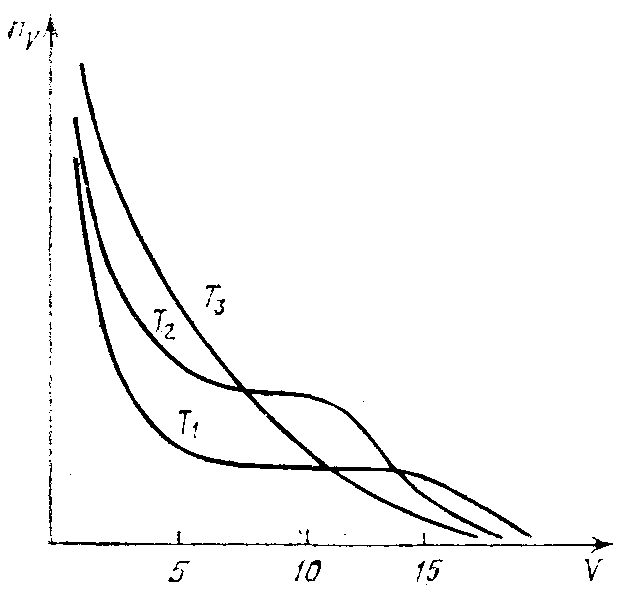
\includegraphics[width=.47\textwidth]{23_1}\hfill
    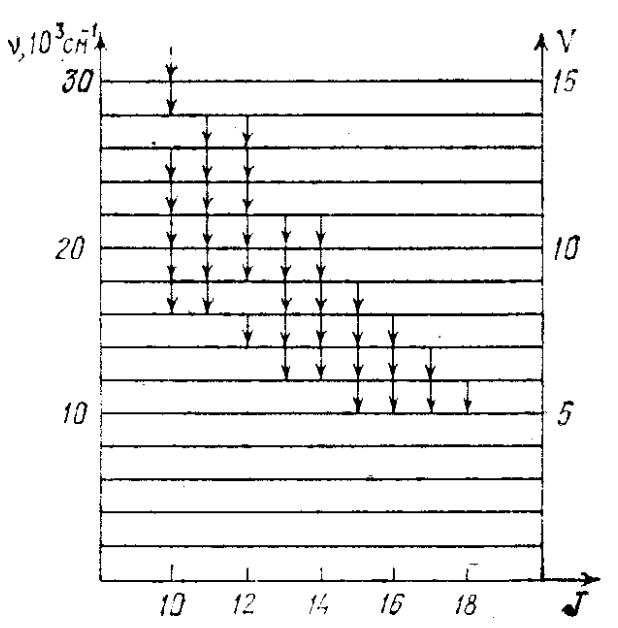
\includegraphics[width=.47\textwidth]{23_2}
    \parbox[t]{.47\textwidth}{\caption{Уровни энергии молекулы \( CO \)}}\hfill
    \parbox[t]{.47\textwidth}{\caption{Каскадные переходы}}
\end{figure}


Суммарный по всем линиям генерации КПД может достигать весьма больших
значений. Возможна работа в импульсном и непрерывном режимах. Применение в
качестве буферного газа ксенона позволяет перейти к комнатной температуре и
отпаянным системам. Характерной особенностью этого лазера является отсутствие
колебательной инверсии и каскадный характер генерации в \( P \)-ветви
колебательно-вращательных переходов.

При температуре кипения жидкого азота возможно получение мощностей
\( \sim 10^2 \)~Вт при КПД около 50\%.
